\newpage
ҒТАМР 31.21.18

\sectionwithauthors{Т.Т.Машан}{ТӨМЕНГІ ҚЫСЫМДАҒЫ КӨМІРСУТЕКТЕРДІҢ ЭЛЕКТР ӨРІСІНДЕ ЖАНУЫН ЗЕРТТЕУ}

\begin{center}
{\bfseries Т.Т.Машан}

Л.Н.Гумилев атындағы Еуразия ұлттық университеті, Астана, Қазақстан

togzhan-mashan@mail.ru
\end{center}

Бензол буының атомдық қатынасы C/O = 1,0 болатын оттегі ортасында
жүйесіндегі P = 40 Торр қысымда, көлемі 10\% аргон қосылғанда жануы
кезінде күйе түзілу процесіне, күйе бөлшектерінің шығымы мен құрылымына
және фуллерен шығымына U = 0,5...20 кВ кернеу диапазонындағы әртүрлі
полярлы электр өрісінің әсері зерттелді. Алынған нәтижелерді талдау
белгілі бір жағдайларда сыртқы электр өрісінің әсері электр өрісін
қолданбаған шығымдылықпен салыстырғанда күйе шығымын (10\%-ға дейін)
арттыруы мүмкін екенін көрсетті. Күйе бөлшектері U≥20 кВ кернеуде теріс
полярлық үшін тепе-теңдік аймағында дислокациямен қалыпты таралу заңымен
көбірек сипатталатыны анықталды. Электр өрісі, жалпы алғанда, өріс
әсерінсіз алынған бөлшектердің орташа өлшемімен салыстырғанда, күйе
бөлшектерінің орташа мөлшерінің ұлғаюына ықпал етеді. Кернеу өзгерген
кезде күйе пакетінің L\textsubscript{a} диаметрінің ұзындығы оның
L\textsubscript{c} биіктігінен жоғарырақ өзгеретіні анықталды.
ИҚ-спектроскопия көмегімен күйе сығындыларында C\textsubscript{60},
C\textsubscript{70} фуллерендер және ПЦАК анықталды. Аномальды жарқырау
разряды аймағында жалынға электр өрісі әсер еткенде фуллерендер шығымы
айтарлықтай арта бастайтыны анықталды (α≥13\%). Күйе үлгілерінің құрғақ
сығындыларының рентгендік фотограммасын талдау С\textsubscript{60} және
С\textsubscript{70} фуллерендеріне тән шыңдардың болуын көрсетті. Шыңдар
фуллерендердің келесі кристалдық фазаларына сәйкес келеді: орторомбты,
кубтық және алтыбұрышты (C\textsubscript{70} тек алтыбұрышты).

{\bfseries Түйін сөздер:} күйе түзілу, фуллерен, экстракция, электр өрісі,
төмен температура, ПЦАК.

\sectionheading{ИССЛЕДОВАНИЕ ГОРЕНИЯ УГЛЕВОДОРОДОВ ПРИ НИЗКОМ ДАВЛЕНИИ В
ЭЛЕКТРИЧЕСКОМ ПОЛЕ}

\begin{center}
{\bfseries Т.Т. Машан}

Евразийский национальный университет им. Л.Н. Гумилева, Астана,
Казахстан,

е-mail: togzhan-mashan@mail.ru
\end{center}

Исследовано влияние постоянного электрического поля различной полярности
на процесс сажеобразования, выход и структуру сажевых частиц, на выход
фуллеренов в диапазоне напряжений U=0,5...20 кВ при сжигании паров
бензола в среде кислорода при атомном соотношении С/О=1,0 с добавлением
10 \% аргона по объему, при давлении в системе Р=40 Торр. Анализ
полученных результатов показал, что воздействие внешнего электрического
поля при определенных условиях может увеличить выход сажи (до 10 \%) по
сравнению с выходом без применения электрического поля. Установлено, что
для частиц сажи наиболее характерен нормальный закон распределения с
дислокацией в зоне равновесия для отрицательной полярности при
напряжении U≥20 кВ. Электрическое поле, в целом, способствует росту
среднего размера частиц сажи по сравнению со средним размером частиц,
полученных без воздействия поля. Установлено, что длина диаметра
сажевого пакета L\textsubscript{a} подвержена большему изменению в
сторону увеличения, чем его высота L\textsubscript{с}, при изменении
напряжения. Методом ИК-спектроскопии в экстрактах сажи идентифицированы
фуллерены С\textsubscript{60}, С\textsubscript{70} и ПЦАУ. Установлено,
что выход фуллеренов значительно начинает расти (α≥13\%) при наложении
на пламя электрического поля в области аномального тлеющего разряда.
Анализ рентгеновской фотограммы сухих экстрактов образцов сажи показал
наличие пиков, характерных для фуллеренов С\textsubscript{60} и
С\textsubscript{70}. Пики соответствуют следующим кристаллическим фазам
фуллеренов: орторомбической, кубической и гексагональной
(C\textsubscript{70} только гексагональная).

{\bfseries Ключевые слова:} сажеобразование, фуллерен, экстракция,
электрическое поле, низкая температура, ПЦАУ.

\sectionheading{STUDY OF HYDROCARBON COMBUSTION AT LOW PRESSURE IN AN ELECTRIC FIELD}

\begin{center}
{\bfseries T.T. Mashan}

L.N. Gumilyov Eurasian National University{\bfseries ,} Astana, Kazakhstan,

е-mail: togzhan-mashan@mail.ru
\end{center}

Influence of a constant electric field of different polarity on
sootformation process, yield and structure of soot particles, on yield
of fullerenes in a range of pressure U=0.5 \ldots{} 20 kV at burning of
benzene vapours in the environment of oxygen at atomic ratio С/О=1.0
with addition of 10 \% of argon on volume, at pressure in system Р=40
Torr is investigated. The analysis of obtained results has shown, that
influence of external electric field under certain conditions can
increase yield of soot (up to 10 \%) in comparison with yield without
applying electric field. It is found that for soot particles most
typical the normal law of distribution with dislocation in the zone of
equilibrium for negative polarity at pressure U≥20 кV. The electric
field, as a whole, promotes growth of the average size soot particles in
comparison with the average size of particles received without field
influence. It is established, that the length of diameter soot package
L\textsubscript{a} is subject to greater change aside increases, than
its height L\textsubscript{с}, at voltage change. Fullerenes
C\textsubscript{60}, С\textsubscript{70} and PAH are identified in
extracts of soot by the method of IR-spectroscopy. It is established,
that yield of fullerenes significantly starts to grow (α≥13\%) at
applying on flame of electric field in the abnormal glow discharge area.
The analysis of X-ray photogram of soot samples dry extracts showed
presence of peaks, characteristic for fullerenes C\textsubscript{60} and
C\textsubscript{70}. Peaks correspond to following crystal phases of
fullerenes: orthorhombic, cubic and hexagonal (C\textsubscript{70} only
hexagonal).

{\bfseries Keywords}: Sootformation, fullerenes, extraction, electrical
field, low pressure, РАН.

\begin{multicols}{2}
{\bfseries Кіріспе.} Күйенің ауылшаруашылығының көптеген салаларында
кеңінен пайдаланылуына байланысты күйе түзілу мәселелері қазіргі заманда
маңыздылыққа ие болып отыр. Қоршаған орта жағдайларында жоғары
тұрақтылық пен ұзақ сақталуға қабылеттілігімен ерекшеленетін күйе
бөлшектері, сонымен қатар, полициклды ароматты көмірсутектер (ПЦАК) де
атмосфераны ластайтын көмірсутек майларын жағу өнімдерінің компоненттері
болып табылатындықтан, экология мәселесі де шиеленісе түсуде. Күйе мен
канцерогенді полициклды ароматты көмірсутектердің шығымын төмендету үшін
қажетті шараларды енгізу, олардың түзілу процесстерін тереңдете
зерттеуді талап етеді.

Жану процесі оң және теріс зарядты иондардың, сондай-ақ, электрондардың
пайда болуымен көрінетін физикалық әсерлермен бірге жүреді {[}1{]}. Күйе
жалындарының құрылымын зерттеу күйе пайда болғанға дейін және оның пайда
болу кезінде болатын химиялық және физикалық процестер туралы құнды
мәліметтер береді, атап айтқанда, қоршаған ортаны бензин мен дизельді
қозғалтқыштардың толық жанбаған өнімдерінен қорғау мәселесіне байланысты
қызығушылық тудырады.

Күйе түзілуін зерттеудің тағы бір маңызды аспектісі - электр өрісінің
жалын құрылымына әсері. Жану процестеріне электр өрісінің әсерін зерттеу
нәтижесінде төмен кернеулі электр өрісін қолдану жану кинетикасына
айтарлықтай әсер ететіні анықталды және көмірсутекті жалындардағы күйе
түзілу процесі көбінесе жалындағы оң зарядталған күйе бөлшегімен
анықталатыны көрсетілді {[}2, 3{]}.

Сыртқы электр өрісінің қолданылуы жалында болатын барлық процестерге:
күйе бөлшектерінің пайда болу процесіне, олардың өсуіне, сонымен қатар,
шөгуіне әсер ететіні белгілі. Күйе бөлшектерінің пайда болуы процесіне
келетін болсақ, иондық теория бар, оған сәйкес
C\textsubscript{n}H\textsubscript{n}\textsuperscript{+} типті иондар
күйе бөлшектерінің өсуінің белсенді орталықтары болып табылады {[}4{]}.
Бөлшектердің мөлшері мен массасы жану аймағында болу уақытымен
анықталады және оны электр өрісін қолдану арқылы өзгертуге болады,
өйткені барлық бөлшектер процестің ең ерте кезеңдерінде зарядтанады.

Атмосфералық қысымда метанның оттегі жалынындағы күйе бөлшектерінің
мөлшеріне және шығым процесіне 0,1-ден 2,2 кВ-қа дейінгі диапазондағы
тұрақты электр өрісінің әсерін анықтау бойынша зерттеулер жүргізілді
{[}5{]}. Полярлығына тәуелсіз электр өрісін қолданғанда, күйе
бөлшектерінің массалық шығымы азайып, олардың мөлшері кішірейіп, күйе
бөлшектерінің құрамы біртекті болатыны анықталды.

Электр өрісінің беттік жануға әсері {[}6{]} сипатталған. Тәжірибелерде
табиғи газ бен ауаның жанғыш қоспасы қолданылған. Қоспаның жануы
матрицаның бетінен жоғары аймақта жүреді. Тәжірибелерде қызықты әсер
анықталған. Электродқа жоғары оң потенциалды қолданғанда, электрод
астындағы аймақта беттік жанудың «бұғатталуы» байқалады. Жарық матрицада
қара дақ пайда болады. Кернеу азайған сайын қараңғы аймақтың көлемі
кішірейеді. Беттік жануды «бұғаттау» әсері екі себепке байланысты болуы
мүмкін: жалын шебінің беттік аймақтан жойылуы немесе иондық желдің қарсы
қысымы әсерінен ағынға жергілікті газ-динамикалық кедергінің жоғарылауы
салдарынан жергілікті жану қуатының төмендеуі.

Тұрақты және импульстік-периодты электр өрісінің пропан-ауа қоспасының
жануына әсері {[}7{]} жұмыста зерттелген. Тәжірибе көрсеткендей, кернеу
берілгенде иондық желдің пайда болуынан жалын пішіні өзгереді.
Ламинарлық жану режимінде тұрақты кернеу 3,4 кВ-қа өзгергенде жалынның
таралу жылдамдығы шамамен 20\%-ға артады. Турбулентті режим үшін бұл
жылдамдық шамамен 30\%-ға артады. Айнымалы кернеу электродына 1 кВ
бергенде, 4 мс ұзақтықтағы импульстарды беру жиілігі 150 Гц-тен бастап
өзгертсе жиіліктің артуы тұрақты өрісті қолданғандағыдай жалынның таралу
жылдамдығының айтарлықтай артуына алып келді. Тәжірибелерде, сонымен
қатар, ламинарлы режимнен турбулентті жану режиміне көшу кезінде
жалынның тұрақтылығына тұрақты электр өрісінің әсері анықталды.

Көмірсутекті жалынға әсер ететін электр өрісі заряд тасымалдаушыларға
электр денесінің күші әсерінен иондық жел тудырады. Иондық жел күйе
шығаруға, жалынның таралу жылдамдығына және жалын тұрақтылығына әсер
ететіні көрсетілген, бірақ иондық желдің егжей-тегжейлі әрекеті және
оның жалынға әсері әлі анық емес. Екі параллель электродтың арасына
орнатылған сопло арқылы өтетін араласпаған және алдын ала араластырылған
жалындарға тұрақты және айнымалы электр өрістерін берген кездегі жалын
мен иондық желдің динамикалық әрекеті зерттелген. Ион желі анодқа да,
катодқа да қарай соғатыны тіркелген және жалын түріне (араластырылмаған
немесе алдын ала араласқан) немесе электр өрісінің көзіне (тұрақты және
айнымалы тоқ) тәуелді емес {[}8{]}.

Маңызды технологиялық шикізат болғандықтан күйе өнеркәсіптік ауқымда
әртүрлі тәсілдермен өндіріледі. Негізінен \textasciitilde1700 К
температурада сұйық және газ тәрізді көмірсутектерді жеткіліксіз оттекте
жағу, содан кейін ыдырау өнімдерін жылдам салқындату арқылы термиялық
ыдырау әдісі қолданылады. Мұндай күйе материалы жеке тұйықталған
бөлшектерден тұрады, мұнда диаметрі ондаған және жүздеген Å болатын
сфералық глобулалар біріншілік болып табылады, олар бір-бірімен химиялық
байланысып, сызықтық тармақталу тізбектері спиральдар, кластерлер және
т.б. сияқты агрегаттарға біріктіріліп, екінші реттік құрылым түзуге
қабілетті {[} 9{]}.

Күйе түзілу механизмі туралы көптеген теориялар мен идеялар бар, күйе
түзілу процесіне келесі аралық өнімдер қатысады: С, С\textsubscript{2},
СН, С\textsubscript{2}Н, СН\textsubscript{2},
С\textsubscript{3}Н\textsubscript{4},
С\textsubscript{4}Н\textsubscript{3}; полиацетилендер
C\textsubscript{4}H\textsubscript{2},
C\textsubscript{6}H\textsubscript{2},
C\textsubscript{10}H\textsubscript{2}; полициклді ароматты
көмірсутектер, сондай-ақ, 1,3-бутадиен немесе винилацетилен сияқты
қосарланған байланыстары бар молекулалар {[}10, 11{]}. Көмірсутекті
газдарды жағу кезінде көміртекті наноқұрылым -- фуллерендер алу
мүмкіндігі анықталған {[}12{]}.

Бұл жұмыста төмен қысымда 0,5-тен 20 кВ-қа дейінгі кернеу диапазонындағы
күйе бөлшектерінің құрылымы мен күйе түзілу процесіне электр өрісінің
әсері зерттелген және түзілген күйе құрамында фуллерендердің болатыны
дәлелденді.

{\bfseries Материалдар мен әдістер.} Зерттеулер бензол буының оттегімен C/O
= 1,0 атомдық қатынасында 10\% аргонды қосу арқылы жануы 40 Торр қысымда
жүргізілді.

Бензол сұйықтыққа арналған шприц тәріздес мөлшерлегіш арқылы 1 мл/мин
мөлшерінде реакторға енгізілді, бұл көлемдік бу шығынының
Q\textsubscript{1} = 250 см\textsuperscript{3}/мин мөлшерін қамтамасыз
етті. Оттегі мен аргон ∆Р = 5 кгс/см\textsuperscript{2} қысымда
редукторлар арқылы берілді және капиллярлық шығын өлшегіштермен
бақыланды. Құрылғының схемасы 1-суретте көрсетілген.
\end{multicols}

\begin{figure}[H]
	\centering
	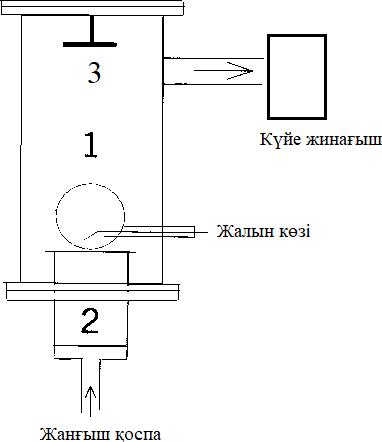
\includegraphics[width=0.5\textwidth]{assets/23}
	\caption*{1-сурет Төменгі қысымда күйе алу жандырғысының схемамы}
\end{figure}

\begin{multicols}{2}
Жанғыш қоспаны дайындау келесі реттілікпен өтті. Сұйық бензол
мөлшерлегіш арқылы буландырғышқа енгізілді, алдын ала таңдалған
температуралық режим оның бірден дерлік булануын қамтамасыз етті.
Түзілген бензол булары буландырғышқа түсетін оттегі мен аргон
молекулаларымен араласып, содан кейін қоспа сифон тәрізді буқыздырғыш
буферлік ыдысқа түсті. Жақсы араластырылу үшін жанғыш қоспаны буферлік
резервуарға ұшы дәнекерленген перфорацияланған түтік арқылы өткізді.
Бу-газ жанғыш қоспасының соңғы дайындығы тікелей инертті материалдан
жасалған шарлармен толтырылған жандырғыда аяқталды. Бензол буларының
конденсациясын болдырмау үшін жанғыш қоспаны беру жолы қыздырылады.
Буферлік ыдыста пайда болған бу-газ қоспасының P\textsubscript{арт} = 13
кПа шегіндегі артық қысымы жанғыш қоспаның жандырғыға біркелкі берілуін
қамтамасыз етеді. Цилиндрлік жандырғының перфорацияланған
тұрақтандырғышынан жанғыш қоспаның шығу жылдамдығы V = 18,38 см/с болды.
Осы жағдайда жалындағы максималды температура T = 1200 К және жалын шебі
жандырғыдан δ = 0,5-0,8 см ажырайтын тұрақты жану туындады. Бір
тәжірибенің ұзақтығы τ = 20 мин. Жану циклі аяқталғаннан кейін кварц
реакторы мен күйе жинағыштың қабырғаларынан күйе жиналып, өлшеніп,
электронды микроскопта және ДРОН -3M дифрактометрінде
(Cu\textsubscript{α} -- сәулелену) зерттелді.

Электродтар арақашықтығы L = 18 см болатын ине-жазықтық электрод жүйесі
кварц реакторында (1) орналастырылған. Жазық электрод - сумен
салқындатылатын жандырғы (2). Ине тәрізді электродқа (3) оң немесе теріс
полярлық 0,5-тен 20 кВ-қа дейінгі диапазондағы тұрақты жоғары вольтты
кернеу берілді. Нәтижесінде жалын аймағын да, жану өнімдерінің аймағын
да қамтитын бойлық электр өрісі пайда болды.

Электр өрісі қолданылған кезде электрондардан, оң және теріс иондардан
тұратын кеңістік зарядын туындататын теріс немесе оң тәж разряды пайда
болды. Кеңістіктік заряд жалын шебіне орналастырылды және жану процесіне
тікелей әсер етті.
\end{multicols}

\begin{figure}[H]
	\centering
	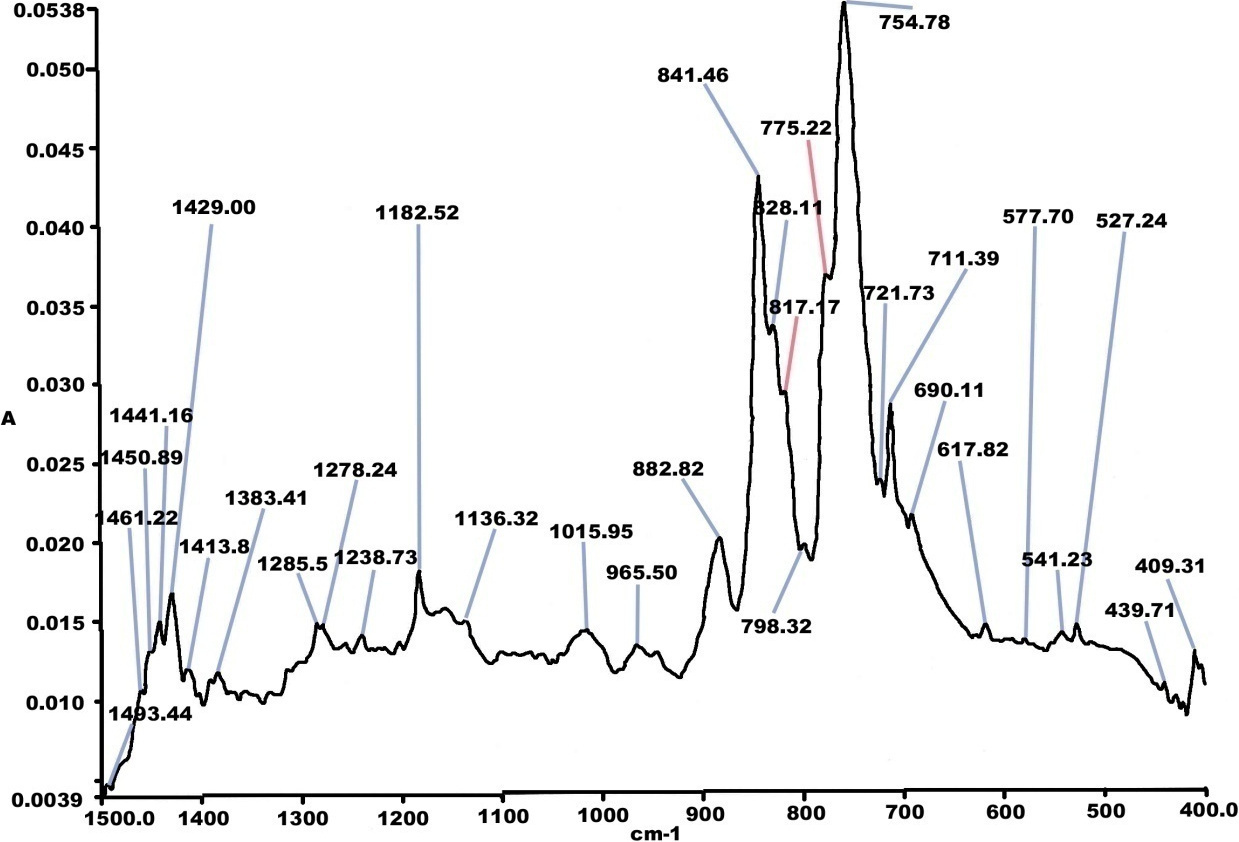
\includegraphics[width=0.8\textwidth]{assets/24}
	\caption*{а) U=1,0 кВ}
\end{figure}

\begin{figure}[H]
	\centering
	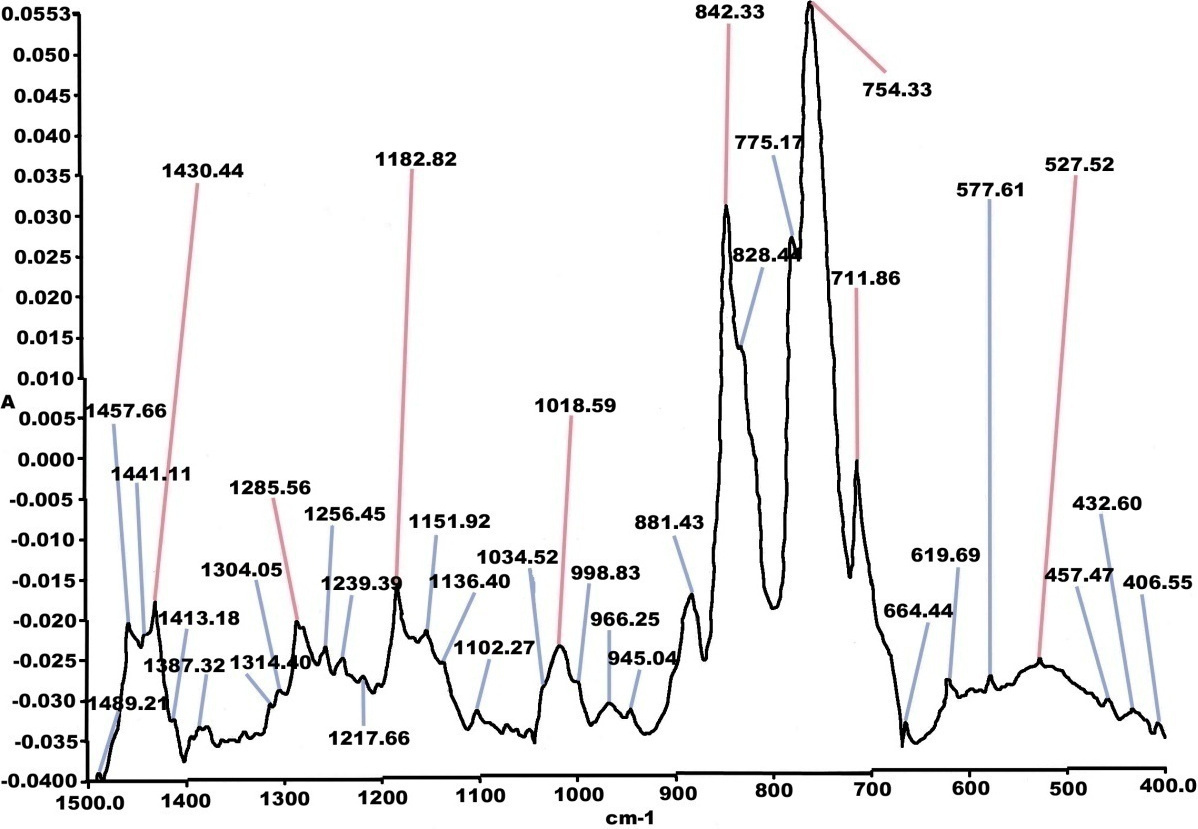
\includegraphics[width=0.7\textwidth]{assets/25}
	\caption*{б) U=2,0 кВ}
\end{figure}

\begin{figure}[H]
	\centering
	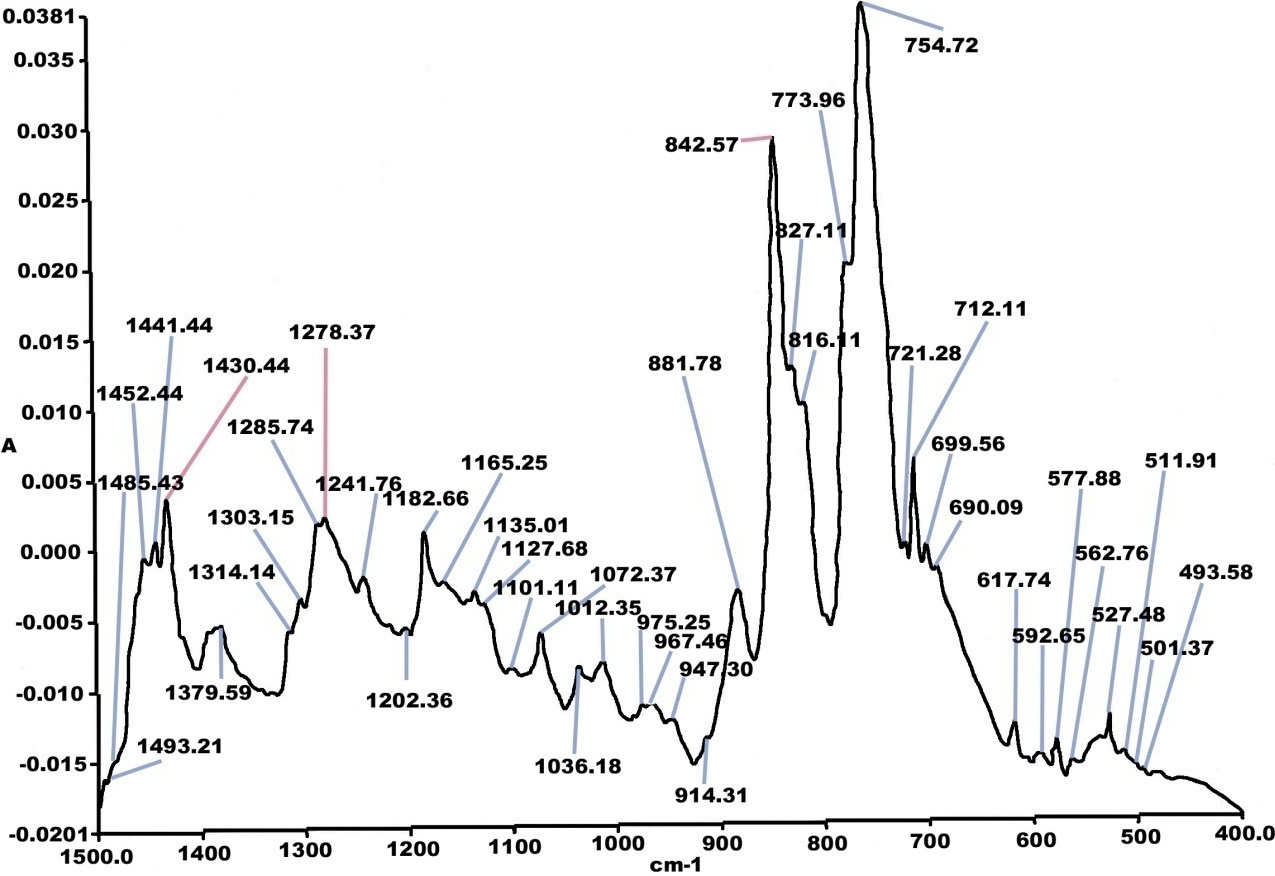
\includegraphics[width=0.7\textwidth]{assets/26}
	\caption*{в) U=20,0 кВ}
	\caption*{2-сурет. Күйе сығындыларының ИҚ спектрлері}
\end{figure}

\begin{figure}[H]
    \centering
    \begin{subfigure}[b]{0.32\textwidth}
        \centering
        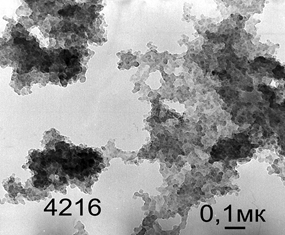
\includegraphics[width=\textwidth]{assets/29}
        \caption*{a)}
    \end{subfigure}
    \hfill
    \begin{subfigure}[b]{0.32\textwidth}
        \centering
        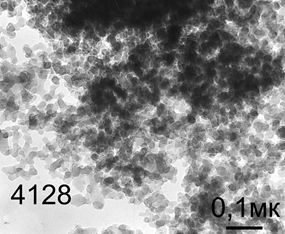
\includegraphics[width=\textwidth]{assets/30}
        \caption*{б)}
    \end{subfigure}
    \hfill
    \begin{subfigure}[b]{0.32\textwidth}
        \centering
        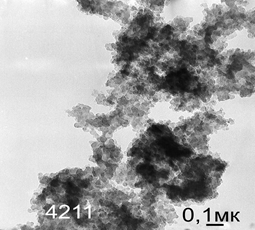
\includegraphics[width=\textwidth]{assets/31}
        \caption*{в)}
    \end{subfigure}
    \caption*{3-сурет. Алынған күйе үлгілері: C/O=1, P=40 Toрр, a) U=0,5 кВ, б) U=1,0 кВ, в) U=2,0 кВ.}
\end{figure}

\begin{multicols}{2}
{\bfseries Нәтижелер} {\bfseries мен талқылау.} Әртүрлі жағдайларда алынған
күйе 72 сағат бойы бензолда суық экстракция әдісімен экстракцияланды.
Сығынды қаныққан қою қызыл түске ие болды, ол ПЦАК пен фуллерендердің
болуына сәйкес келеді. Содан кейін сығынды ИҚ-Фурье спектрометрі
көмегімен талданды. Күйе сығындысы қабықшасының ИҚ жұтылу спектрі 3050
см\textsuperscript{-1}-де жұтылу ароматты сақиналардың С-Н
байланыстарына сәйкес екенін көрсетті. 2960, 2870, 1470, 1390
см\textsuperscript{-1} жұтылу жолақтары CH\textsubscript{2} және
CH\textsubscript{3} функционалдық топтарындағы C-H тербелістік
байланыстарына сәйкес келеді. 1600 см\textsuperscript{-1} спектрі
ароматты сақинаның С=С байланыстарына сәйкес келеді. Сондай-ақ, С=О және
С-С байланыстарына сәйкес келетін жұту жолақтары бар. Спектрлерден
фуллерендердің болатыны да байқалады. Электр өрісін беру арқылы алынған
күйе сығындыларының спектрлері 2-суретте, а, б, в көрсетілген: а) U=1
кВ, б) U=2,0 кВ, в) U=20,0 кВ.

1-кестеде ПЦАК және С\textsubscript{60} және С\textsubscript{70}
фуллерендеріне сәйкес тәжірибелік жолмен алынған және эталондық ИҚ
спектрлері көрсетілген.
\end{multicols}

\begin{table}[H]
\caption*{1-кесте. ПЦАК және фуллерендердің тәжірибелік және эталондық спектрлерін салыстыру}
\centering
\begin{tabular}{|lll|}
\hline
\multicolumn{1}{|l|}{Фуллерендер} & \multicolumn{1}{l|}{Тәжірибелік , $\lambda$ см-1} & Эталон, $\lambda$ см-1 \\ \hline
\multicolumn{1}{|l|}{С60} & \multicolumn{1}{l|}{528, 578, 1183, 1429} & 528, 577,  1183, 1429 \\ \hline
\multicolumn{1}{|l|}{С70} & \multicolumn{1}{p{0.3\textwidth}|}{457, 538, 563, 578, 679, 798, 1136, 1414, 1430, 1460} & \multicolumn{1}{p{0.3\textwidth}|}{458, 535, 565, 578, 642, 674, 795, 1134, 1414, 1430, 1460} \\ \hline
\multicolumn{3}{|c|}{ПЦАК} \\ \hline
\multicolumn{1}{|l|}{Пирен} & \multicolumn{1}{l|}{711, 755, 842, 1183} & 710, 750, 840, 1190 \\ \hline
\multicolumn{1}{|l|}{Флуорантен} & \multicolumn{1}{l|}{618, 755, 775, 827} & 615, 750, 775, 825 \\ \hline
\multicolumn{1}{|l|}{Коронен} & \multicolumn{1}{l|}{543, 842, 1314} & 545, 850, 1313 \\ \hline
\multicolumn{1}{|l|}{Антантрен} & \multicolumn{1}{l|}{690, 775, 880} & 690, 762, 877 \\ \hline
\multicolumn{1}{|l|}{1,12-бензперилен} & \multicolumn{1}{l|}{755, 775, 817, 842} & 645, 750, 765, 817, 845 \\ \hline
\end{tabular}
\end{table}

\begin{table}[H]
\caption*{2-кесте. Электр өрісін қолданған кездегі рентген құрылымдық сипаттамалар және күйе шығымы}
\centering
\begin{tabular}{|l|l|l|l|l|l|l|}
\hline
№ & U, кВ & Өрістердің орналасуы & $L_a$, Å & $L_c$, Å & $d_{002}$, Å & $m_k$,г \\ \hline
1. & Өріссіз & - & 38,13 & 9,42 & 3,71 & 0,5839 \\ \hline
2. & 0,5 & $\pm$ & 31,64 & 8,16 & 3,71 & 0,4633 \\ \hline
3. & 1,1 & $\pm$ & 65,71 & 10,0 & 3,71 & 0,4848 \\ \hline
4. & 2,05 & $\pm$ & 65,7 & 11,41 & 3,71 & 0,5270 \\ \hline
5. & 3,05 & $\pm$ & 57,5 & 11,86 & 3,70 & 0,3784 \\ \hline
6. & 10 & $\pm$ & 57,5 & 11,86 & 3,70 & 0,3322 \\ \hline
7. & 20 & $\pm$ & 57,5 & 11,4 & 3,87 & 0,3631 \\ \hline
8. & 0,5 & $\pm$ & 52,33 & 8,66 & 3,71 & 0,4632 \\ \hline
9. & 1,1 & $\pm$ & 52,07 & 9,58 & 3,69 & 0,6216 \\ \hline
10. & 2,05 & $\pm$ & 65,7 & 12,71 & 3,70 & 0,4695 \\ \hline
11. & 3,05 & $\pm$ & 49,73 & 13,09 & 3,65 & 0,3752 \\ \hline
12. & 10 & $\pm$ & 49,73 & 12,0 & 3,78 & 0,3167 \\ \hline
13. & 20 & $\pm$ & 40,0 & 9,67 & 3,70 & 0,4070 \\ \hline
\end{tabular}
\end{table}

\begin{multicols}{2}
Әртүрлі электр өрістерінде алынған күйе үлгілері үшін рентгендік
дифракциялық сипаттамалары және күйенің массалық шығымы анықталды
(2-кесте). Рентген сәулелерінің дифракциялық үлгілері бойынша үлгі
бөлшектері түзілетін күйе пакетінің құрылымын сипаттайтын
L\textsubscript{a}, L\textsubscript{c}, d\textsubscript{002} когерентті
шашырау аймағының мәндері есептелді. Мұндағы L\textsubscript{a} -- күйе
пакетінің диаметрінің ұзындығы, L\textsubscript{c} -- биіктігі,
d\textsubscript{002} -- күйе пакетіндегі екі қабат арасындағы қашықтық.

Кестеден көрініп тұрғандай, полярлықты өзгерту күйе бөлшектерінің шығымы
мен мөлшеріне қатты әсер етеді.

Күйе үлгілерінің микроэлектрондық кескіндері алынды, 2-сурет. 0,5-тен 2
кВ-қа дейінгі электр өрісін қолданғанда, алынған күйе үлгілерінің
өлшемдері 261 Å-ден 334 Å-ге дейін өзгерді.

Бұл зерттеулерде қолданылатын электр өрісінің полярлығына қарамастан
электродаралық қашықтықтығы L = 18 см ине-жазықтық электродтарындағы тәж
разряды (газ аралығының жартылай тесілуі) U = 10 кВ дейін сақталды.
Кернеу U = 10 кВ және одан жоғары болған кезде, тәж разряды катод мен
анодты қосатын жарқыраған, ирек жіңішке жіптің пайда болуымен солғын
электр разрядына айналды. Бірақ жалын шебіне солғын электр разрядын
қабат орналастырған кезде, жарқыраған жіп жалынға сіңіп, электродқа
(жандырғыға) жетпей қалды.

Электр өрісінің жалынға әсері теріс полярлық үшін U ≥ 1,35 кВ бастап
(жоғарғы ине-электродта минус) және оң полярлық үшін U ≥ 3,0 кВ (жоғарғы
ине-электродта плюс) визуалды түрде байқалды. Көзге көрінетін әсері
жалынның сығылуымен, тербелісімен, созылуымен, жалпаюымен, қызғалдақ
пішініне айналуымен және басқа да құбылыстардан байқалды. Электр өрісі
болмаған кезде жалын тұрақты, тербеліссіз жанып тұрды, d = 2,5 см, жарық
аймағының биіктігі h = 4,5 см, жандырғыдан бөліну δ = 0,5 см
параметрлері бар цилиндр (жандырғы) пішініне ие болды. Электр өрісін,
мысалы, U = 10 кВ кернеу қолданғанда, жалынның жоғарғы бөлігі толқын
тәрізді тербелетін қызғалдақ тәріздес түрге ие болады.

Осы жұмыста жалынға әсері зерттелген электр өрісі кернеулерінің
диапазонын тиімділігіне қарай шартты түрде екі аймаққа бөлуге болады: I
аймақ - 0,5-тен 3,0 кВ-қа дейін; II аймақ -- 3,0 кВ жоғары.

Бірінші аймақта, күйе шығымы бойынша оң немесе теріс полярлықтың
«тиімділігі» айтарлықтай ерекшеленбейді және күйенің шығу процесі кейде
сәтті, кейде сәтсіз өтті. Бұл жағдайда белгілі бір кернеудегі электр
өрісін қолданғанда күйенің массалық шығымы өріс қолданбағандағы массалық
шығымнан төмен болады. Бұл процесте электр өрісі жану процесіне
каталитикалық әсер береді, сонымен қатар, электр өрісі көмірсутекті
отынның ұзын тізбектерін үзетін күш болып табылады деген гипотезаға
сәйкес келеді.

Алайда, бірінші аймақта электр өрісі кернеулерінің диапазоны
эксперименталды түрде анықталды, оның аймағында күйе түзілудің жоғары
көрсеткіші (шыңы) орын алды және күйенің массалық шығымдылығы (10\%
дейін) электр өрісінің әсерінсіз күйенің шығуынан асып кетті.
Қайталанатын тәжірибелер келтірілген кернеудің полярлығына қарамастан U
= 1,0...1,35 кВ кернеу диапазонында орналасқан жоғарыда келтірілген
тәжірибелік жағдайларда шыңның болуын растады. Бірдей тәжірибелік
жағдайларда күйенің массалық шығымының қайталану қателігі ∆ =1÷ 5 \%
шегінде болды.

Сыртқы электр өрісін берген кезде белсенді орталықтарды пиролиз
аймағынан алып кететін немесе ұстап қалатын күйе түзілу процесі мен
электрлік күштер арасында бәсекелестік әрекеттесу пайда болады және бұл
күйе түзілу кинетикасы үшін ең қолайлы жағдай деп болжауға болады.

Бұл жағдайда берілген кернеудің нәтижесінде күйе бөлшектерінің өсуіне
алып келетін белсенді орталықтар болып табылатын оң
C\textsubscript{n}H\textsubscript{n}\textsuperscript{+} иондарының үлкен
ағыны пиролиз аймағын кесіп өтеді. Берілген кернеудің белгілі бір шектік
мәнінде иондар газ ағынының осьтік компонентасына қатысты қозғалыссыз
деп саналады. Бұл жағдайда күйе бөлшектерінің түзілу жылдамдығы өріс жоқ
жағдаймен салыстырғанда бірнеше есе артады және пиролиз аймағында көзбен
бақыланатын күйе бөлшектері пайда болады. Ұқсас нәтижелер теріс зарядтар
ағынымен де (оң полярлық) алынды.

Берілген кернеулердің екінші аймағында (U \textgreater{} 3 кВ)
полярлыққа қарамастан, U = 3 кВ кернеуіндегі күйе шығымымен
салыстырғанда күйенің массалық шығымының біртіндеп артуы байқалды.
Алайда, жалпы күйе шығымы электр өрісі болмаған жағдайдан төмен болып
қала берді. Бұл кезде күйенің максималды шығымының шыңы байқалмады.
Белсенді орталықтардың түзілуі физикалық және химиялық процестерге
сәйкес келеді, сондықтан бұл аймақта күйе түзілудің мұндай әрекетінің
себебі, мүмкін, қайта зарядталудың термоэлектрондық эмиссияға қарағанда
басым болуынан және белсенді заттардың пиролиз аймағынан шығып кетуінен
туындайды.

{\bfseries Қорытынды.}

1. Зерттеулер көрсеткендей, күрделі құрамды жалынға сыртқы электр
өрісінің әсері жалында болатын процестерді, сондай-ақ, күйе түзілу
процесін бақылауға, сонымен қатар, белгілі бір жағдайларда күйенің
шығымын арттыруға мүмкіндік береді.

2. ИҚ спектроскопиясының көмегімен күйеде фуллерендер
C\textsubscript{60}, C\textsubscript{70} және полициклды ароматтық
көмірсутектер анықталды.

3. С\textsubscript{60} және С\textsubscript{70} фуллерендеріне сәйкес
келетін толқын ұзындықтары оң полярлықпен салыстырғанда теріс полярлықта
айқынырақ анықталғаны көрсетілді. Бұл теріс полярлықтың фуллерендер
шығымына оң полярлыққа қарағанда көбірек әсер ететінін растайды.

4. Спектрлердің интенсивтілігіне сүйене отырып, берілген кернеудің
жоғарылауымен фуллерендердің шығымы жоғарылайтыны анықталды.
\end{multicols}

\begin{center}
{\bfseries Әдебиеттер}
\end{center}

\begin{noparindent}
1. Ильюшонок А.В., Гончаренко И.А., Лешенюк Н.С., Кулешов В.К.,
Терешенков В.И.

О влиянии электрического поля на процесс горения. //Вестник Университета
гражданской защиты МЧС Беларуси. 2019. - Т.3( 2) - С.127-137.

2. Степанов Е.М., Дьячков Б.Г. Ионизация в пламени и электрическое поле.
- М.: Металлургия, 1968. - 312 с.

3. Лаутон Дж., Вайнберг Ф. Электрические аспекты горения. Пер. с англ.
Под общ. ред В.А. Попова. - М.: Энергия, 1976. - 296 с.

4. Крестинин А.В., Кислов М.Б., Раевский А.В. и др. K вопросу о
механизме образования сажевых частиц //Кинетика и катализ, 2000. -
Т.41.(1). - С.102-111.

5. Mansurov Z.A., Merkulov A.A., Popov V.T., Tuleutaev B.K., Almazov
N.S. Ultradispersed carbon black formation during methane combustion in
electric field //Khimiya Tverdogo Topliva. 1994. -- Vol. 3. - С. 83-86.

6. Шмелев В.М. О воздействии электрического поля на поверхностное
горение//Химическая физика.- 2016. - Т.35(2).- С. 33-40.

7. Mansurov Z.A., Chenchyk D., Tuleutaev B.K., Mashan T.T. Soot
formation in diffusion flames of acetylene-alkane//International
Symposium on Combustion Abstracts of Works-in-Progress Posters. 2002.
--P.184.

8. Park, D.G., Chung, S.H., Cha, M.S. Visualization of ionic wind in
laminar jet flames. // Combustion and Flame.- 2017.- Vol.184. -
Р.246-248. DOI 10.1016/j.combustflame.2017.06.011.

9. Березкин В.И. Фуллерены как зародыши сажевых частиц. //Физика
твердого тела, 2000. - № 42(3). - С.567-572.

10. Mansurov Z.A. Cool sooting flames of hydrocarbons. //Journal of
Thermal Science.- 2001. - Vol. 10(3). -P.269-280. DOI
10.1007/s11630-001-0031-8

11. Машан Т.Т. Низкотемпературное сажеобразование при горении пропана /
International Scientific and Practical Conference on "Current Problems
of the Chemistry of Coordination Compounds". Bukhara, Uzbekistan.
22-23-december 2022. - P. 488-492.

12. Galeev I.G., Asadullin T.Y. Obtaining fullerene-containing soot
during combustion of gaseous hydrocarbons in an external electric field.
//Journal of Physics Conference Series. VII Conference on low
temperature plasma in the processes of functional coating preparation.
--2016.-Vol.669(1):012016. DOI 10.1088/1742-6596/669/1/012016
\end{noparindent}

\begin{center}
{\bfseries References}
\end{center}

\begin{noparindent}
1. Il\textquotesingle jushonok A.V., Goncharenko I.A., Leshenjuk N.S.,
Kuleshov V.K., Tereshenkov V.I.

O vlijanii jelektricheskogo polja na process gorenija. //Vestnik
Universiteta grazhdanskoj zashhity MChS Belarusi. 2019. - T.3( 2) -
S.127-137.{[}in Russ.{]}

2.Stepanov E.M., D\textquotesingle jachkov B.G. Ionizacija v plameni i
jelektricheskoe pole. - M.: Metallurgija, 1968. - 312 s. {[}in Russ.{]}

3.Lauton Dzh., Vajnberg F. Jelektricheskie aspekty gorenija. Per. s
angl. Pod obshh. red V.A. Popova. - M.: Jenergija, 1976. - 296 s.{[}in
Russ.{]}

4.Krestinin A.V., Kislov M.B., Raevskij A.V. i dr. K voprosu o mehanizme
obrazovanija sazhevyh chastic //Kinetika i kataliz, 2000. - T.41.(1). -
S.102-111. {[}in Russ.{]}

5. Mansurov Z.A., Merkulov A.A., Popov V.T., Tuleutaev B.K., Almazov
N.S. Ultradispersed carbon black formation during methane combustion in
electric field //Khimiya Tverdogo Topliva. 1994. -- Vol. 3. - С. 83-86.

6. Shmelev V.M. O vozdejstvii jelektricheskogo polja na poverhnostnoe
gorenie//Himicheskaja fizika.- 2016. - T.35(2).- S. 33-40.{[}in Russ.{]}

7. Mansurov Z.A., Chenchyk D., Tuleutaev B.K., Mashan T.T. Soot
formation in diffusion flames of acetylene-alkane//International
Symposium on Combustion Abstracts of Works-in-Progress Posters.- 2002.
-P.184.

8. Park, D.G., Chung, S.H., Cha, M.S. Visualization of ionic wind in
laminar jet flames. // Combustion and Flame.- 2017.-Vol.184. -
Р.246-248. DOI 10.1016/j.combustflame.2017.06.011.

9.Berezkin V.I. Fullereny kak zarodyshi sazhevyh chastic. //Fizika
tverdogo tela, 2000. - №.42(3). - S.567-572

10. Mansurov Z.A. Cool sooting flames of hydrocarbons. //Journal of
Thermal Science.- 2001. - Vol. 10(3). -P.269-280. DOI
10.1007/s11630-001-0031-8

11. Mashan T.T. Nizkotemperaturnoe sazheobrazovanie pri gorenii propana
/ International Scientific and Practical Conference on "Current Problems
of the Chemistry of Coordination Compounds". Bukhara, Uzbekistan.
22-23-december 2022. - P. 488-492.{[}in Russ.{]}

12. Galeev I.G., Asadullin T.Y. Obtaining fullerene-containing soot
during combustion of gaseous hydrocarbons in an external electric field.
//Journal of Physics Conference Series. VII Conference on low
temperature plasma in the processes of functional coating preparation.
--2016.-Vol.669(1):012016. DOI 10.1088/1742-6596/669/1/012016
\end{noparindent}

\emph{{\bfseries Авторлар туралы мәліметтер}}

\begin{noparindent}
Машан Т.Т.- химия ғылымдарының кандидаты, химия кафедрасының профессор
м.а., Л.Н. Гумилев атындағы Еуразия ұлттық университеті, Астана,
Қазақстан, e-mail: togzhan-mashan@mail.ru
\end{noparindent}

\emph{{\bfseries Information about the authors}}

\begin{noparindent}
Mashan T.T.- Candidate of Chemical Sciences, Acting Professor of the
Department of Chemistry, L.N. Gumilyov Eurasian National University,
Astana, Kazakhstan, e-mail: togzhan-mashan@mail.ru
\end{noparindent}
